\section{Grundglieder \skript{25ff, 202-206}}
	\subsection{statische Glieder \skript{28}}
		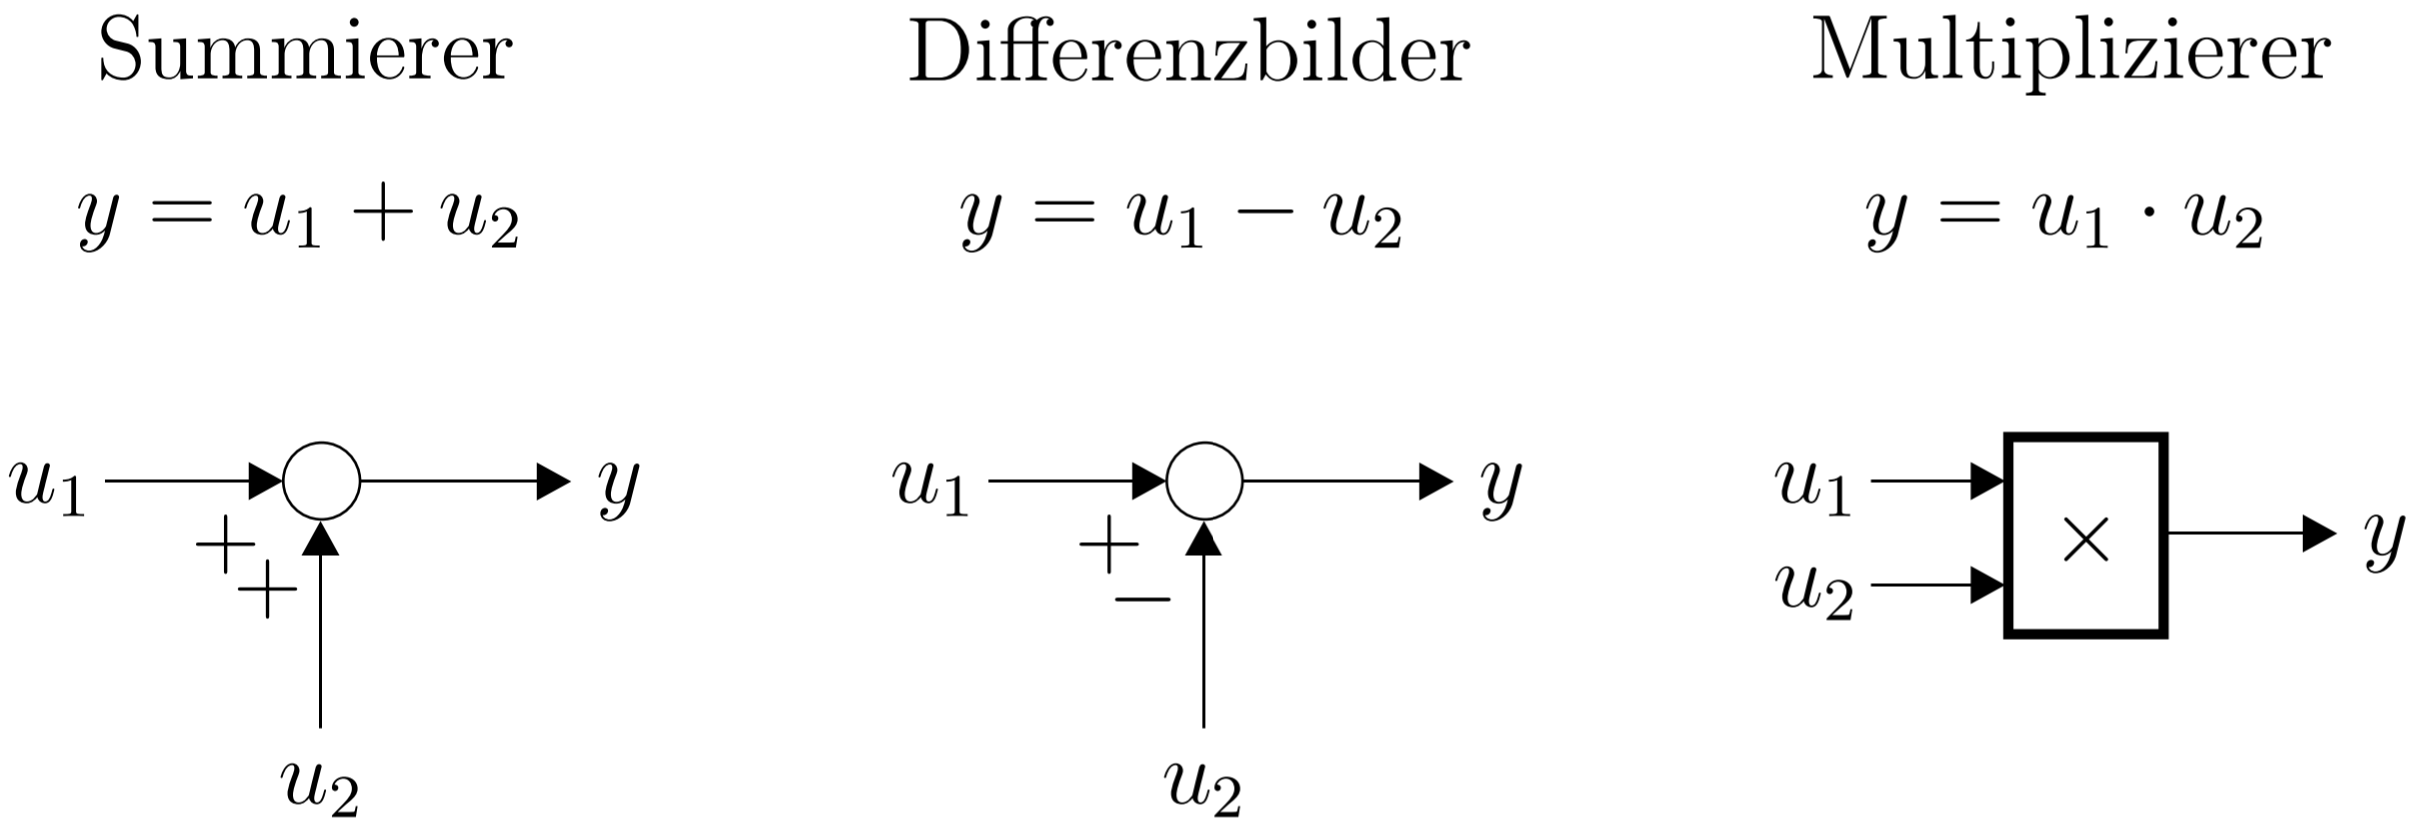
\includegraphics[width=10 cm]{./bilder/grundglieder/statischeGlieder.png} \\
	
	\subsection{dynamische Glieder \skript{25-41, 202-206}}
%		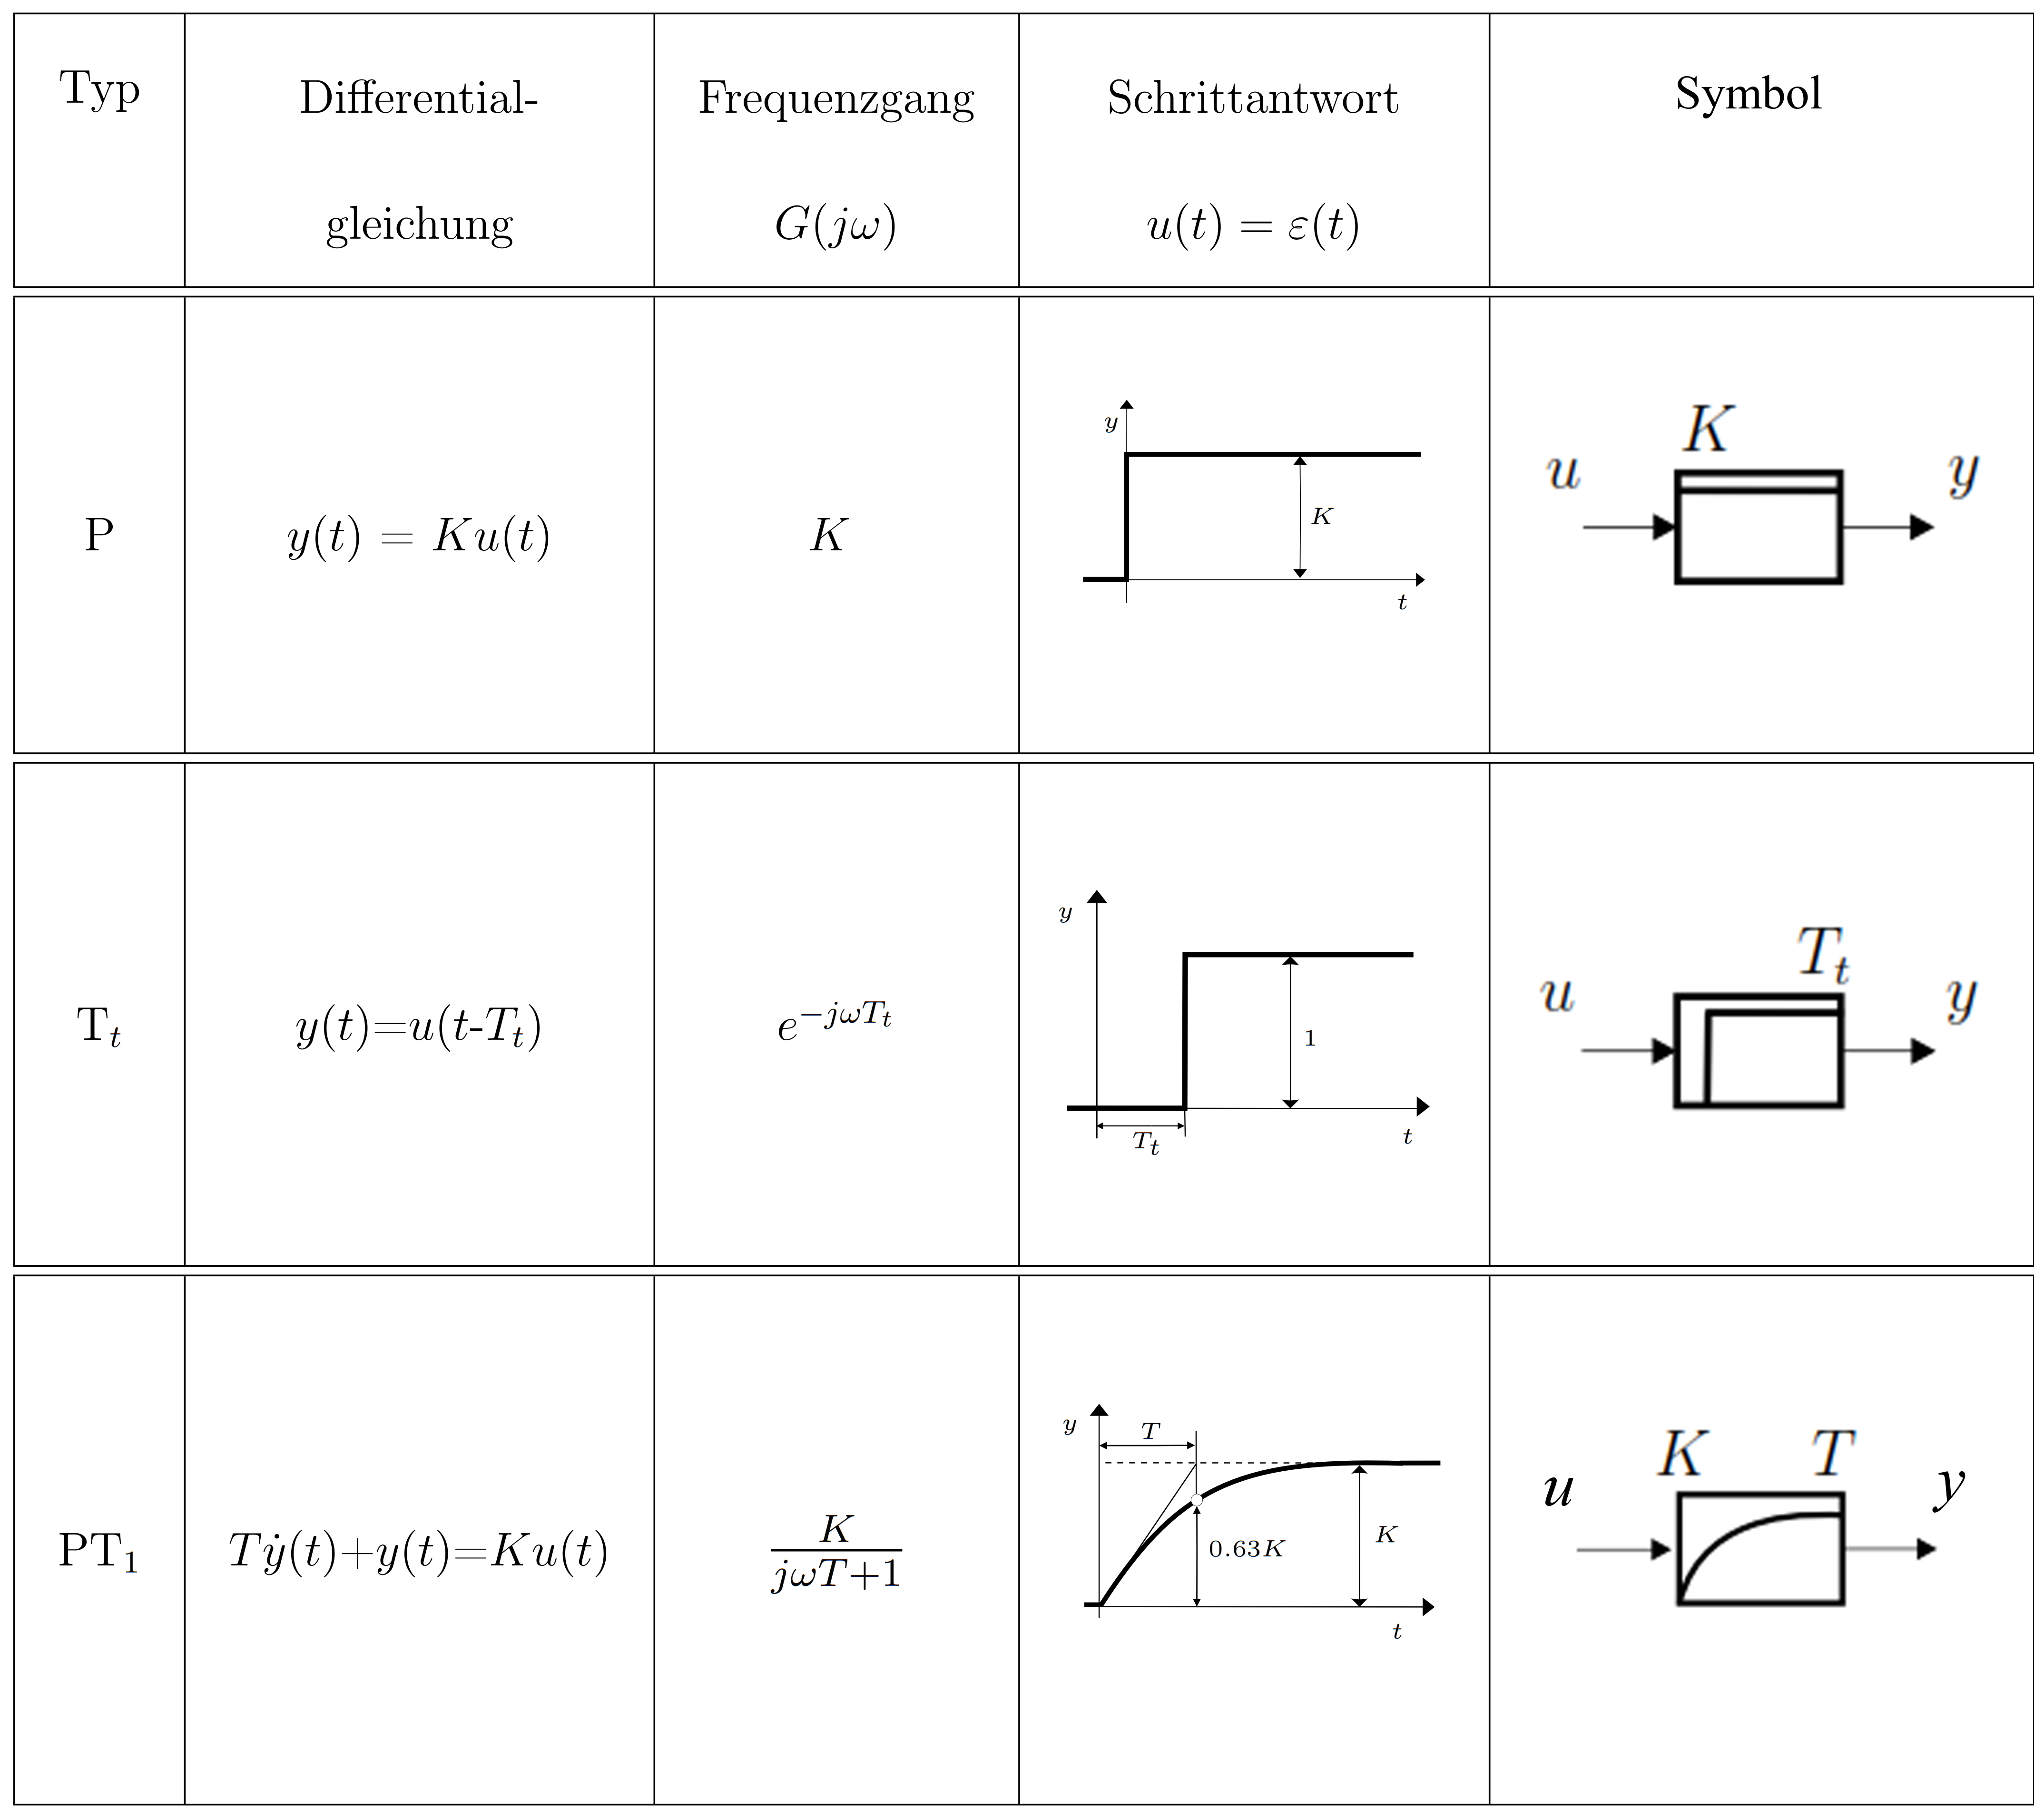
\includegraphics[width=13.5 cm]{./bilder/grundglieder/glieder1.png} \\
%		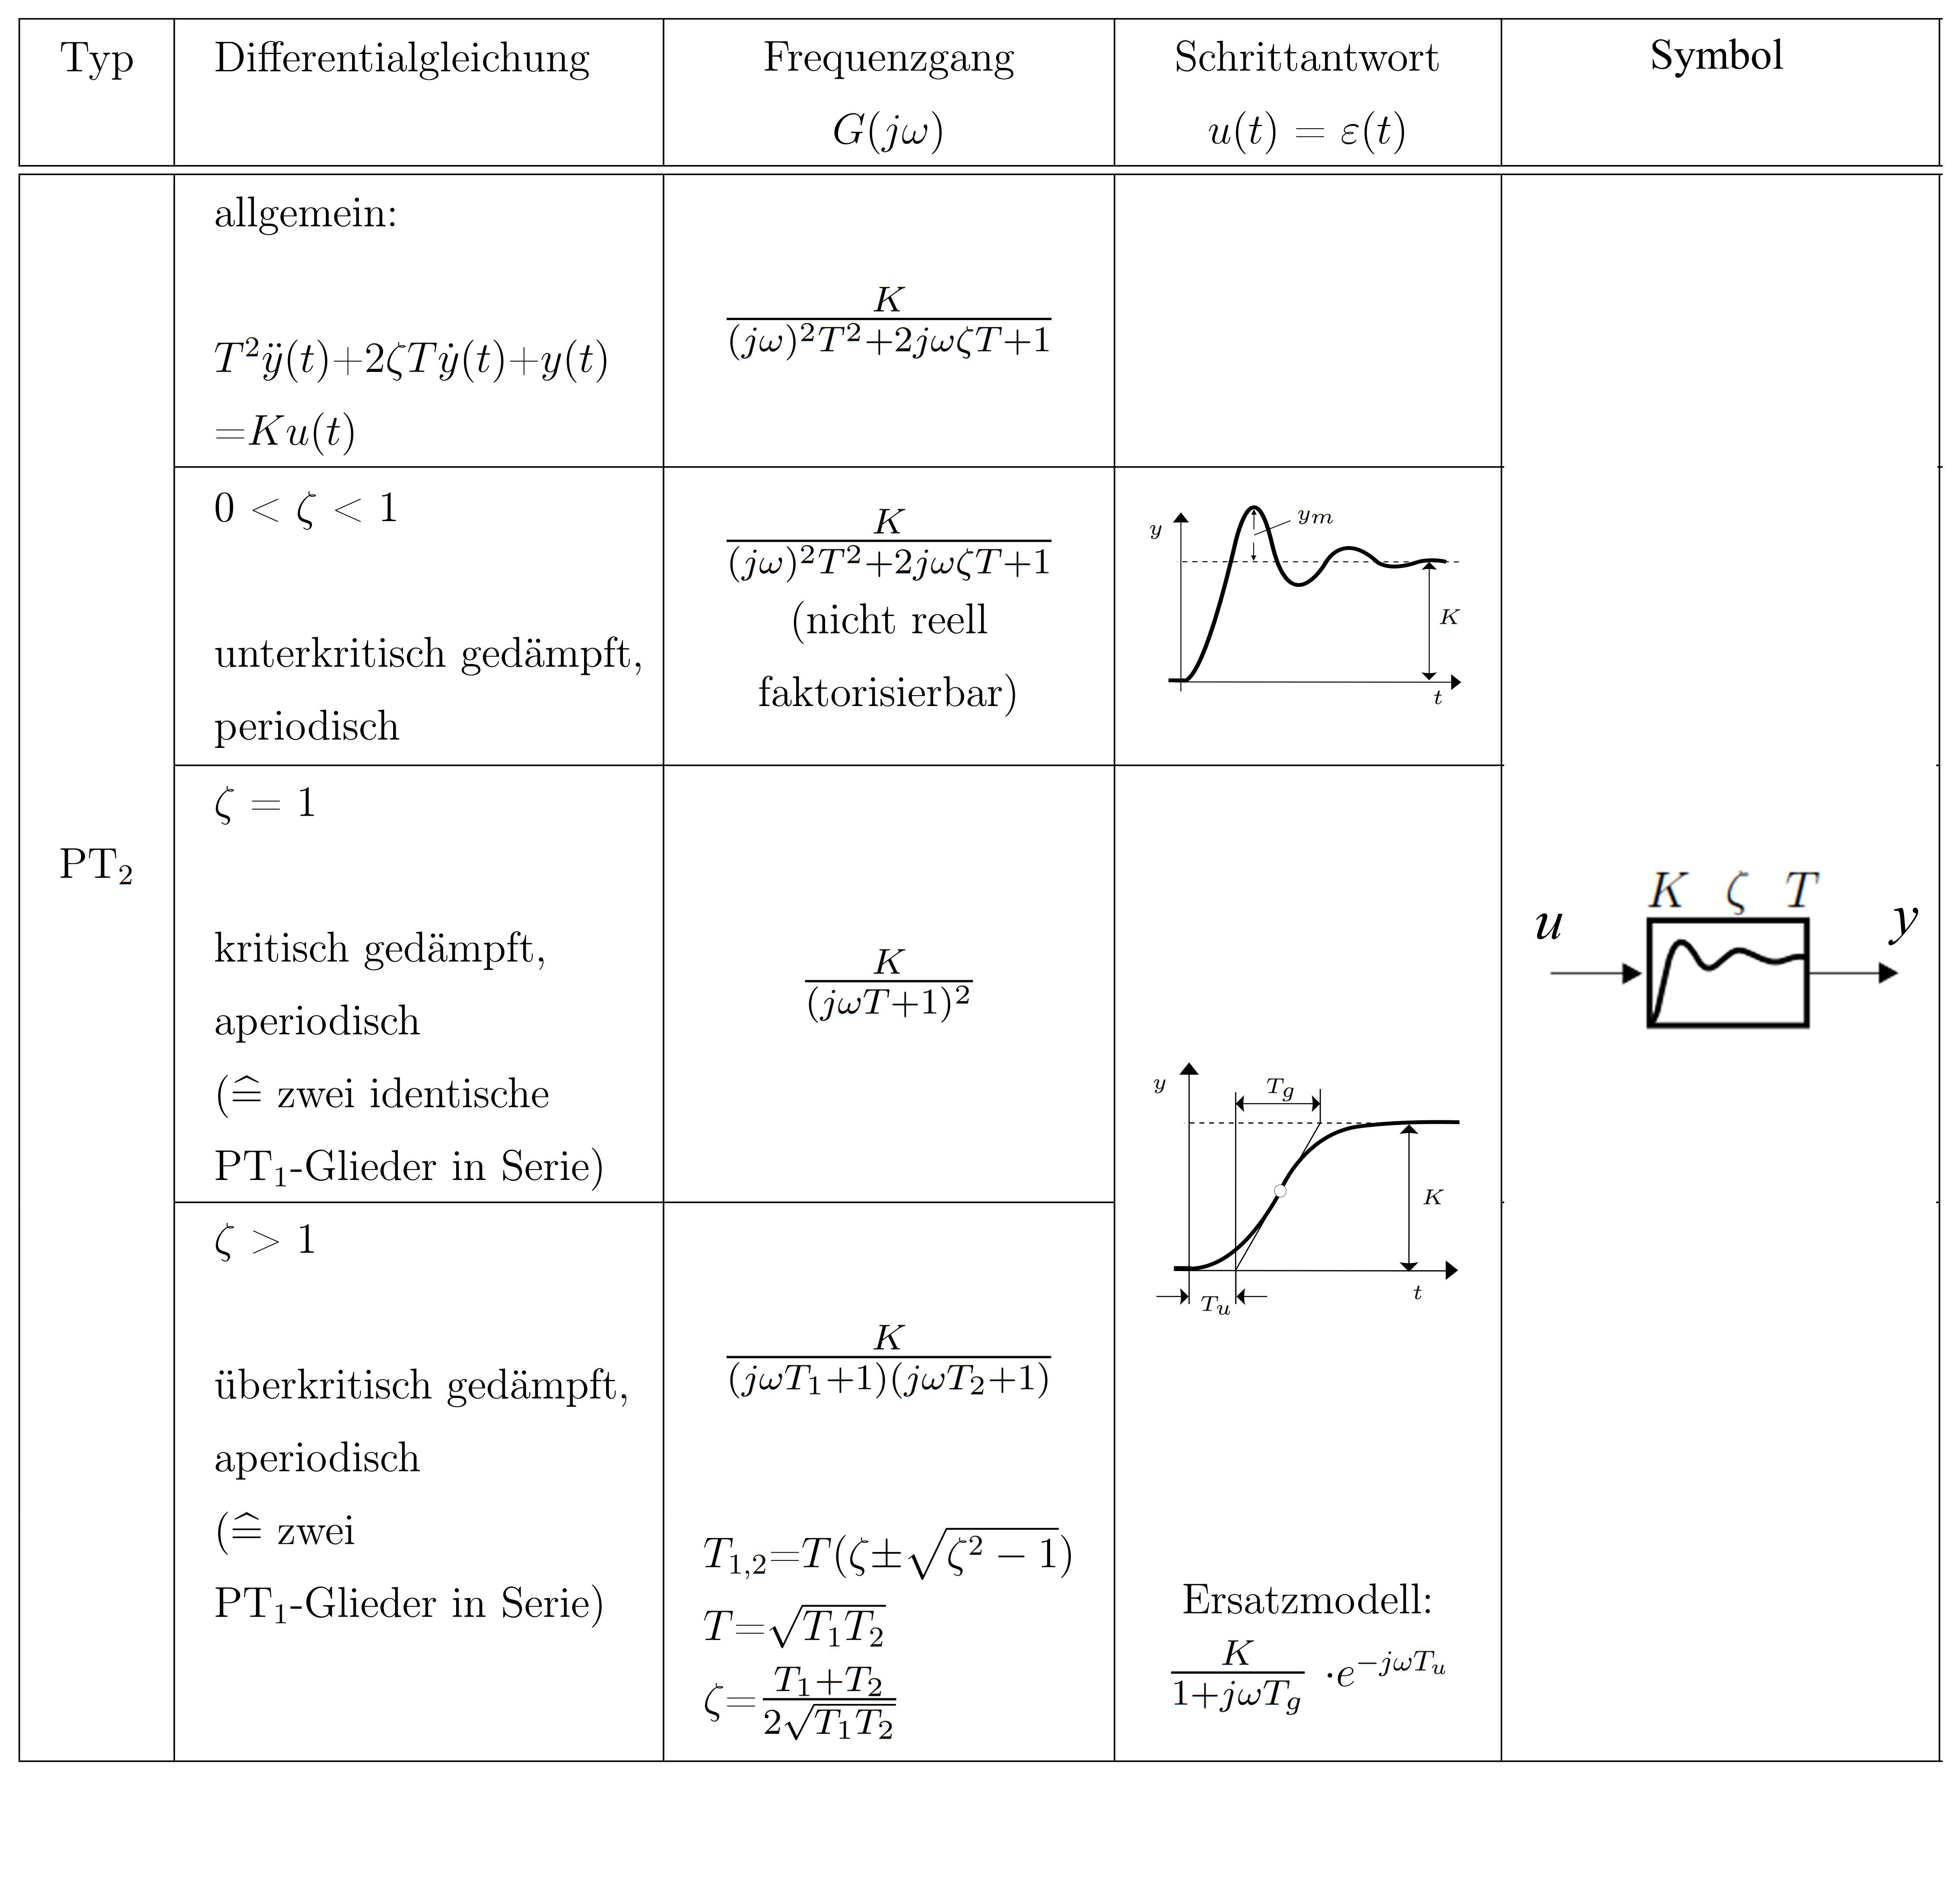
\includegraphics[width=13.5 cm]{./bilder/grundglieder/glieder2.png} \\
%		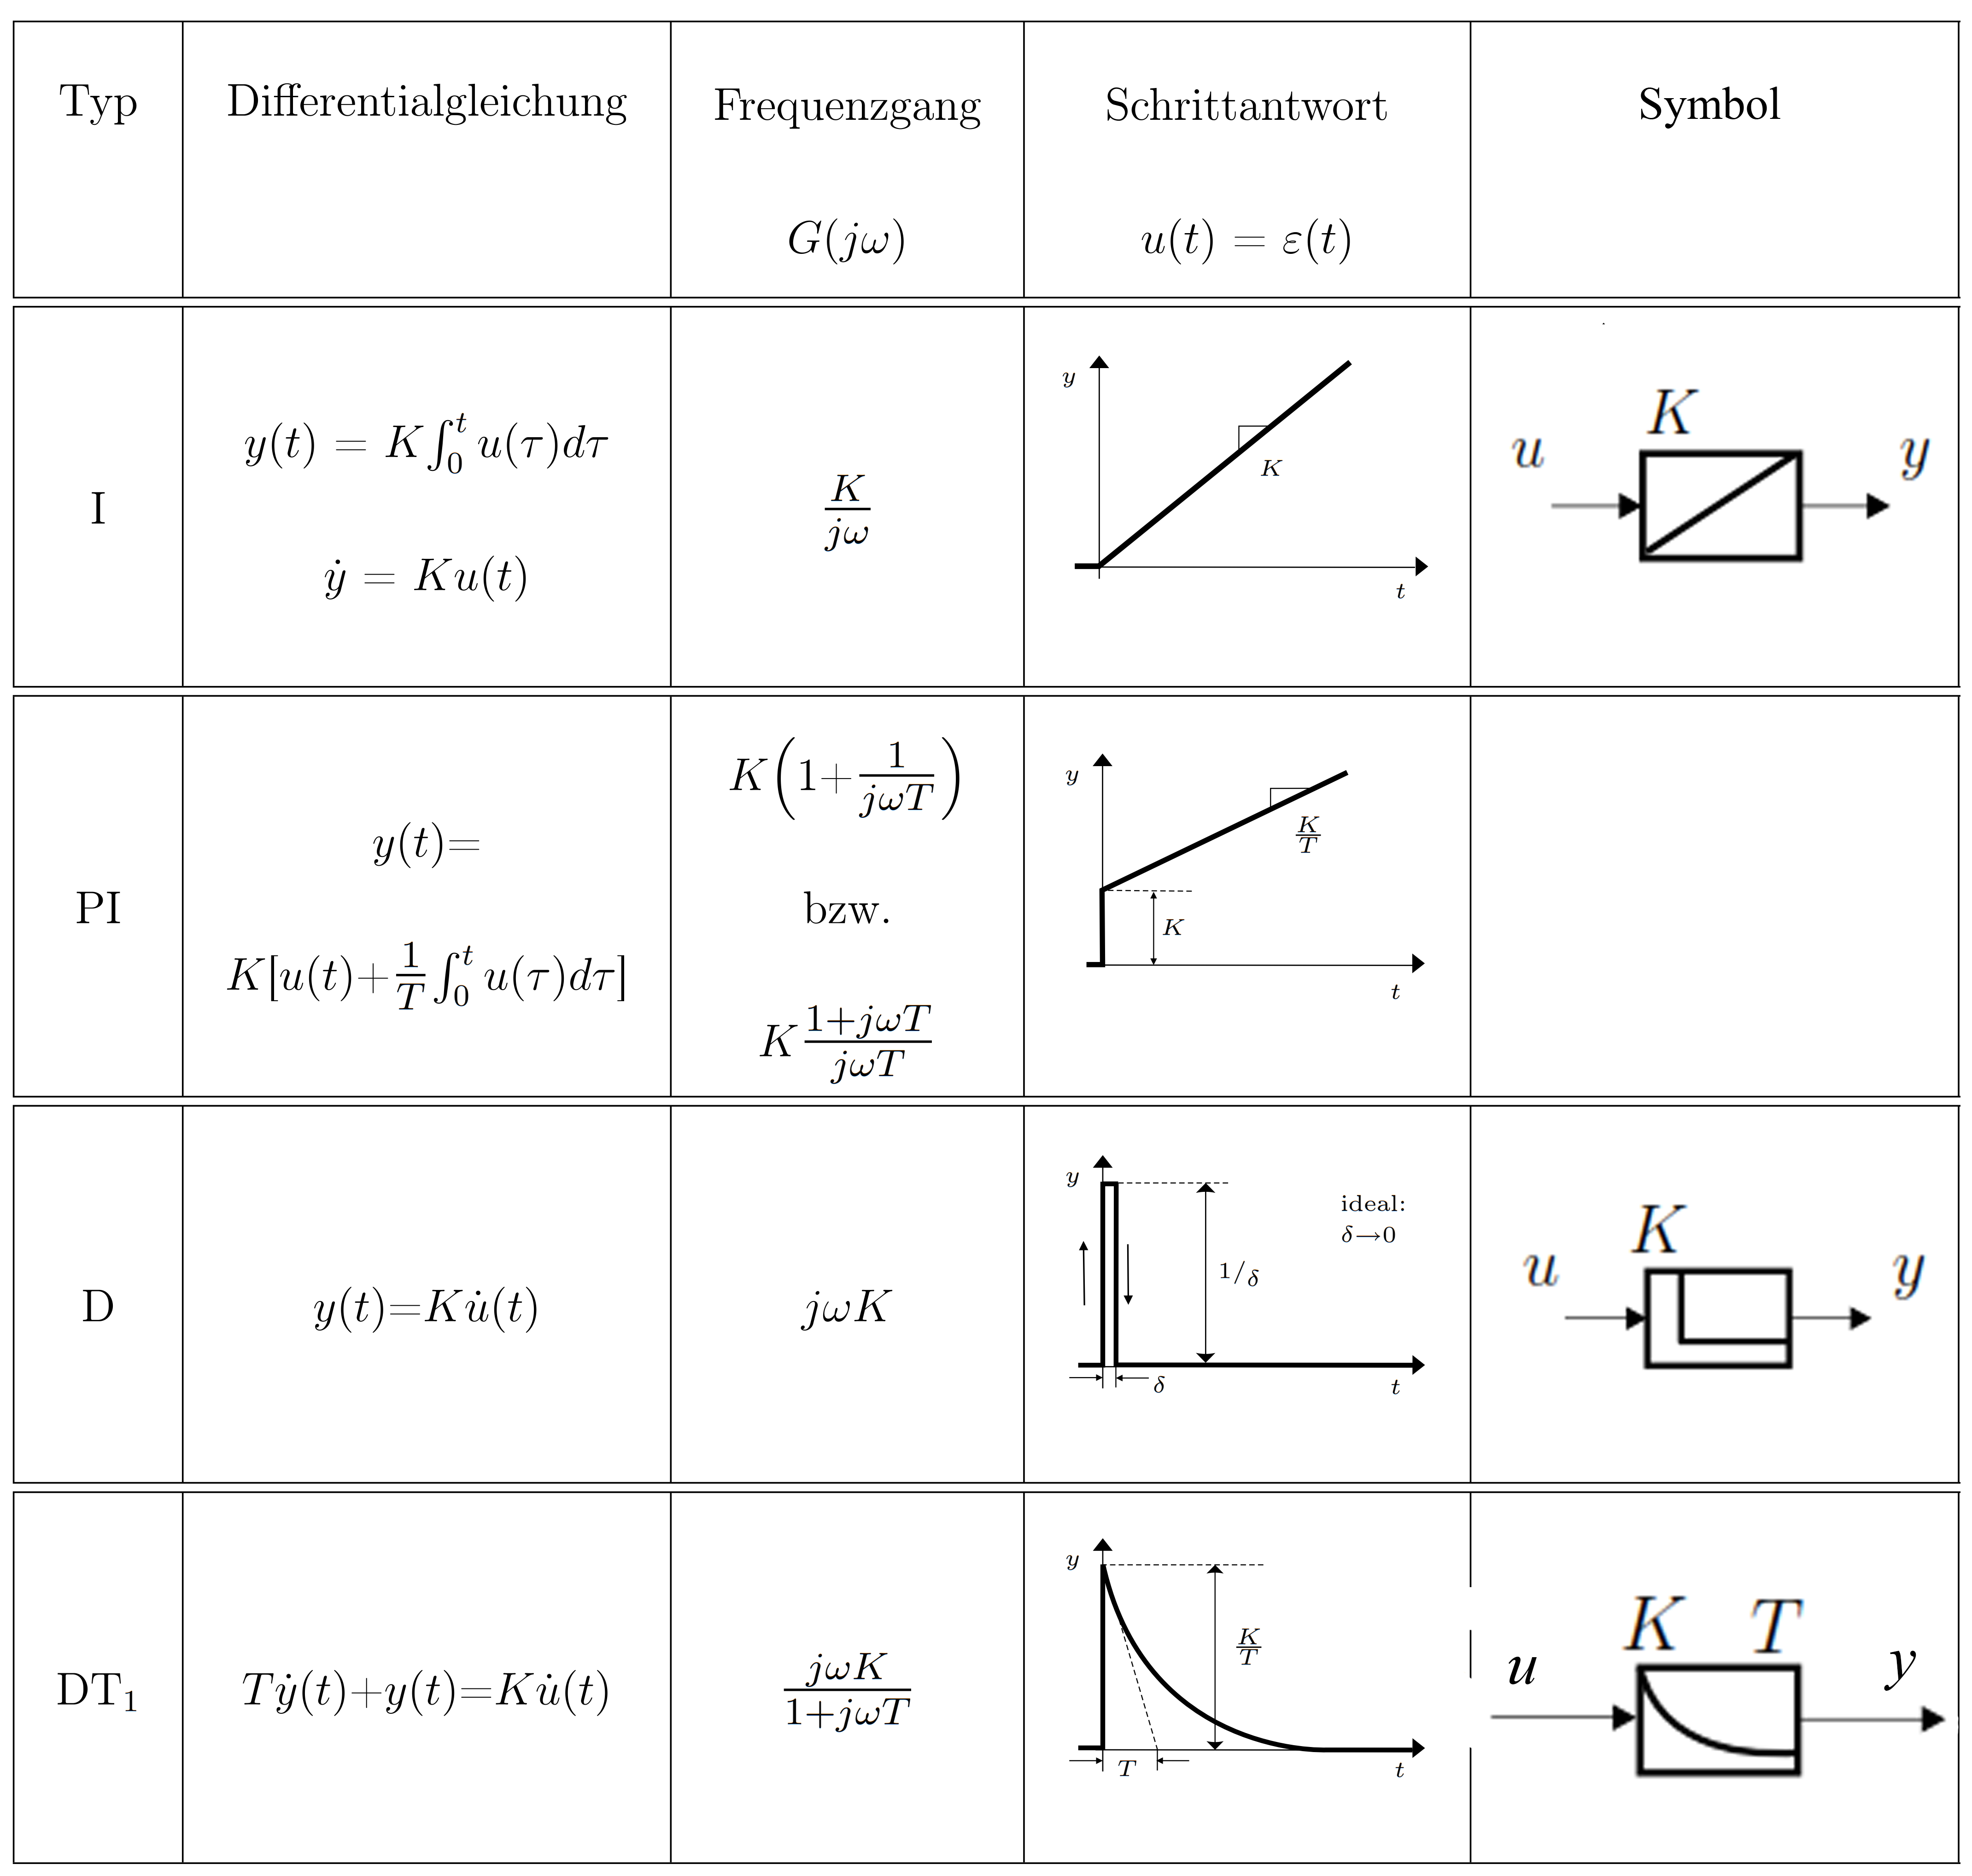
\includegraphics[width=13.5 cm]{./bilder/grundglieder/glieder3.png} \\
%		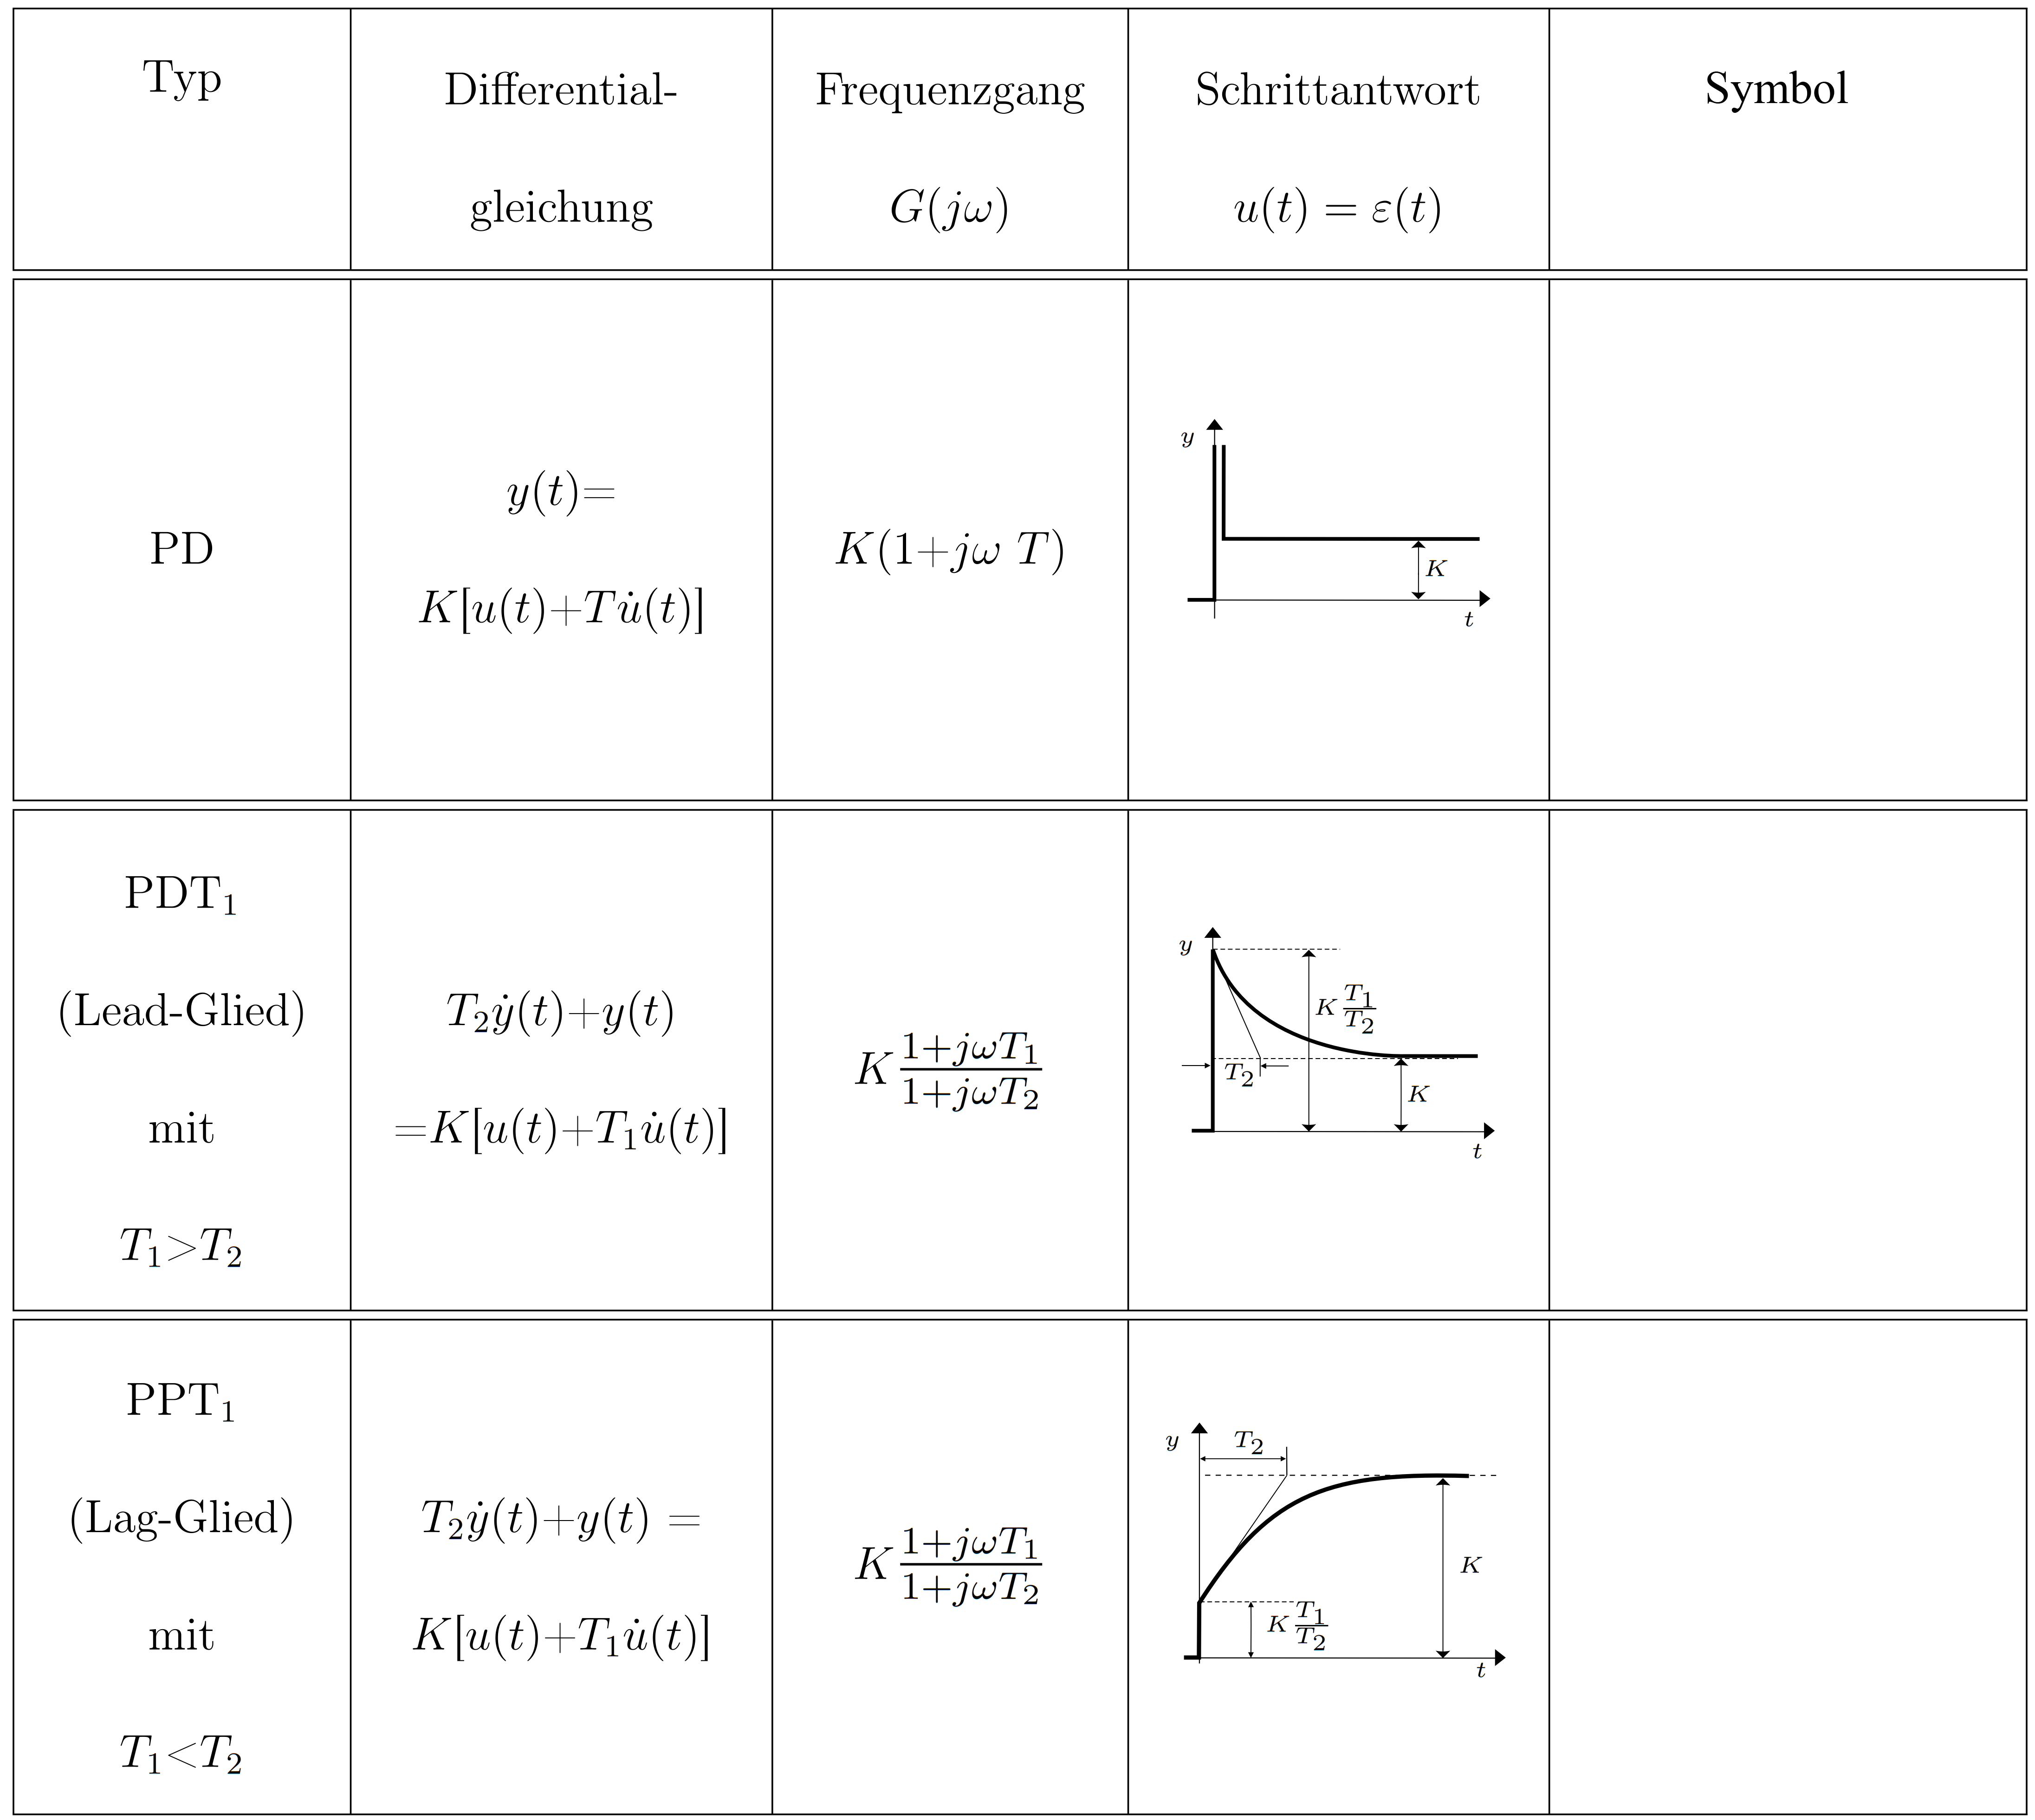
\includegraphics[width=13.5 cm]{./bilder/grundglieder/glieder4.png} \\
%		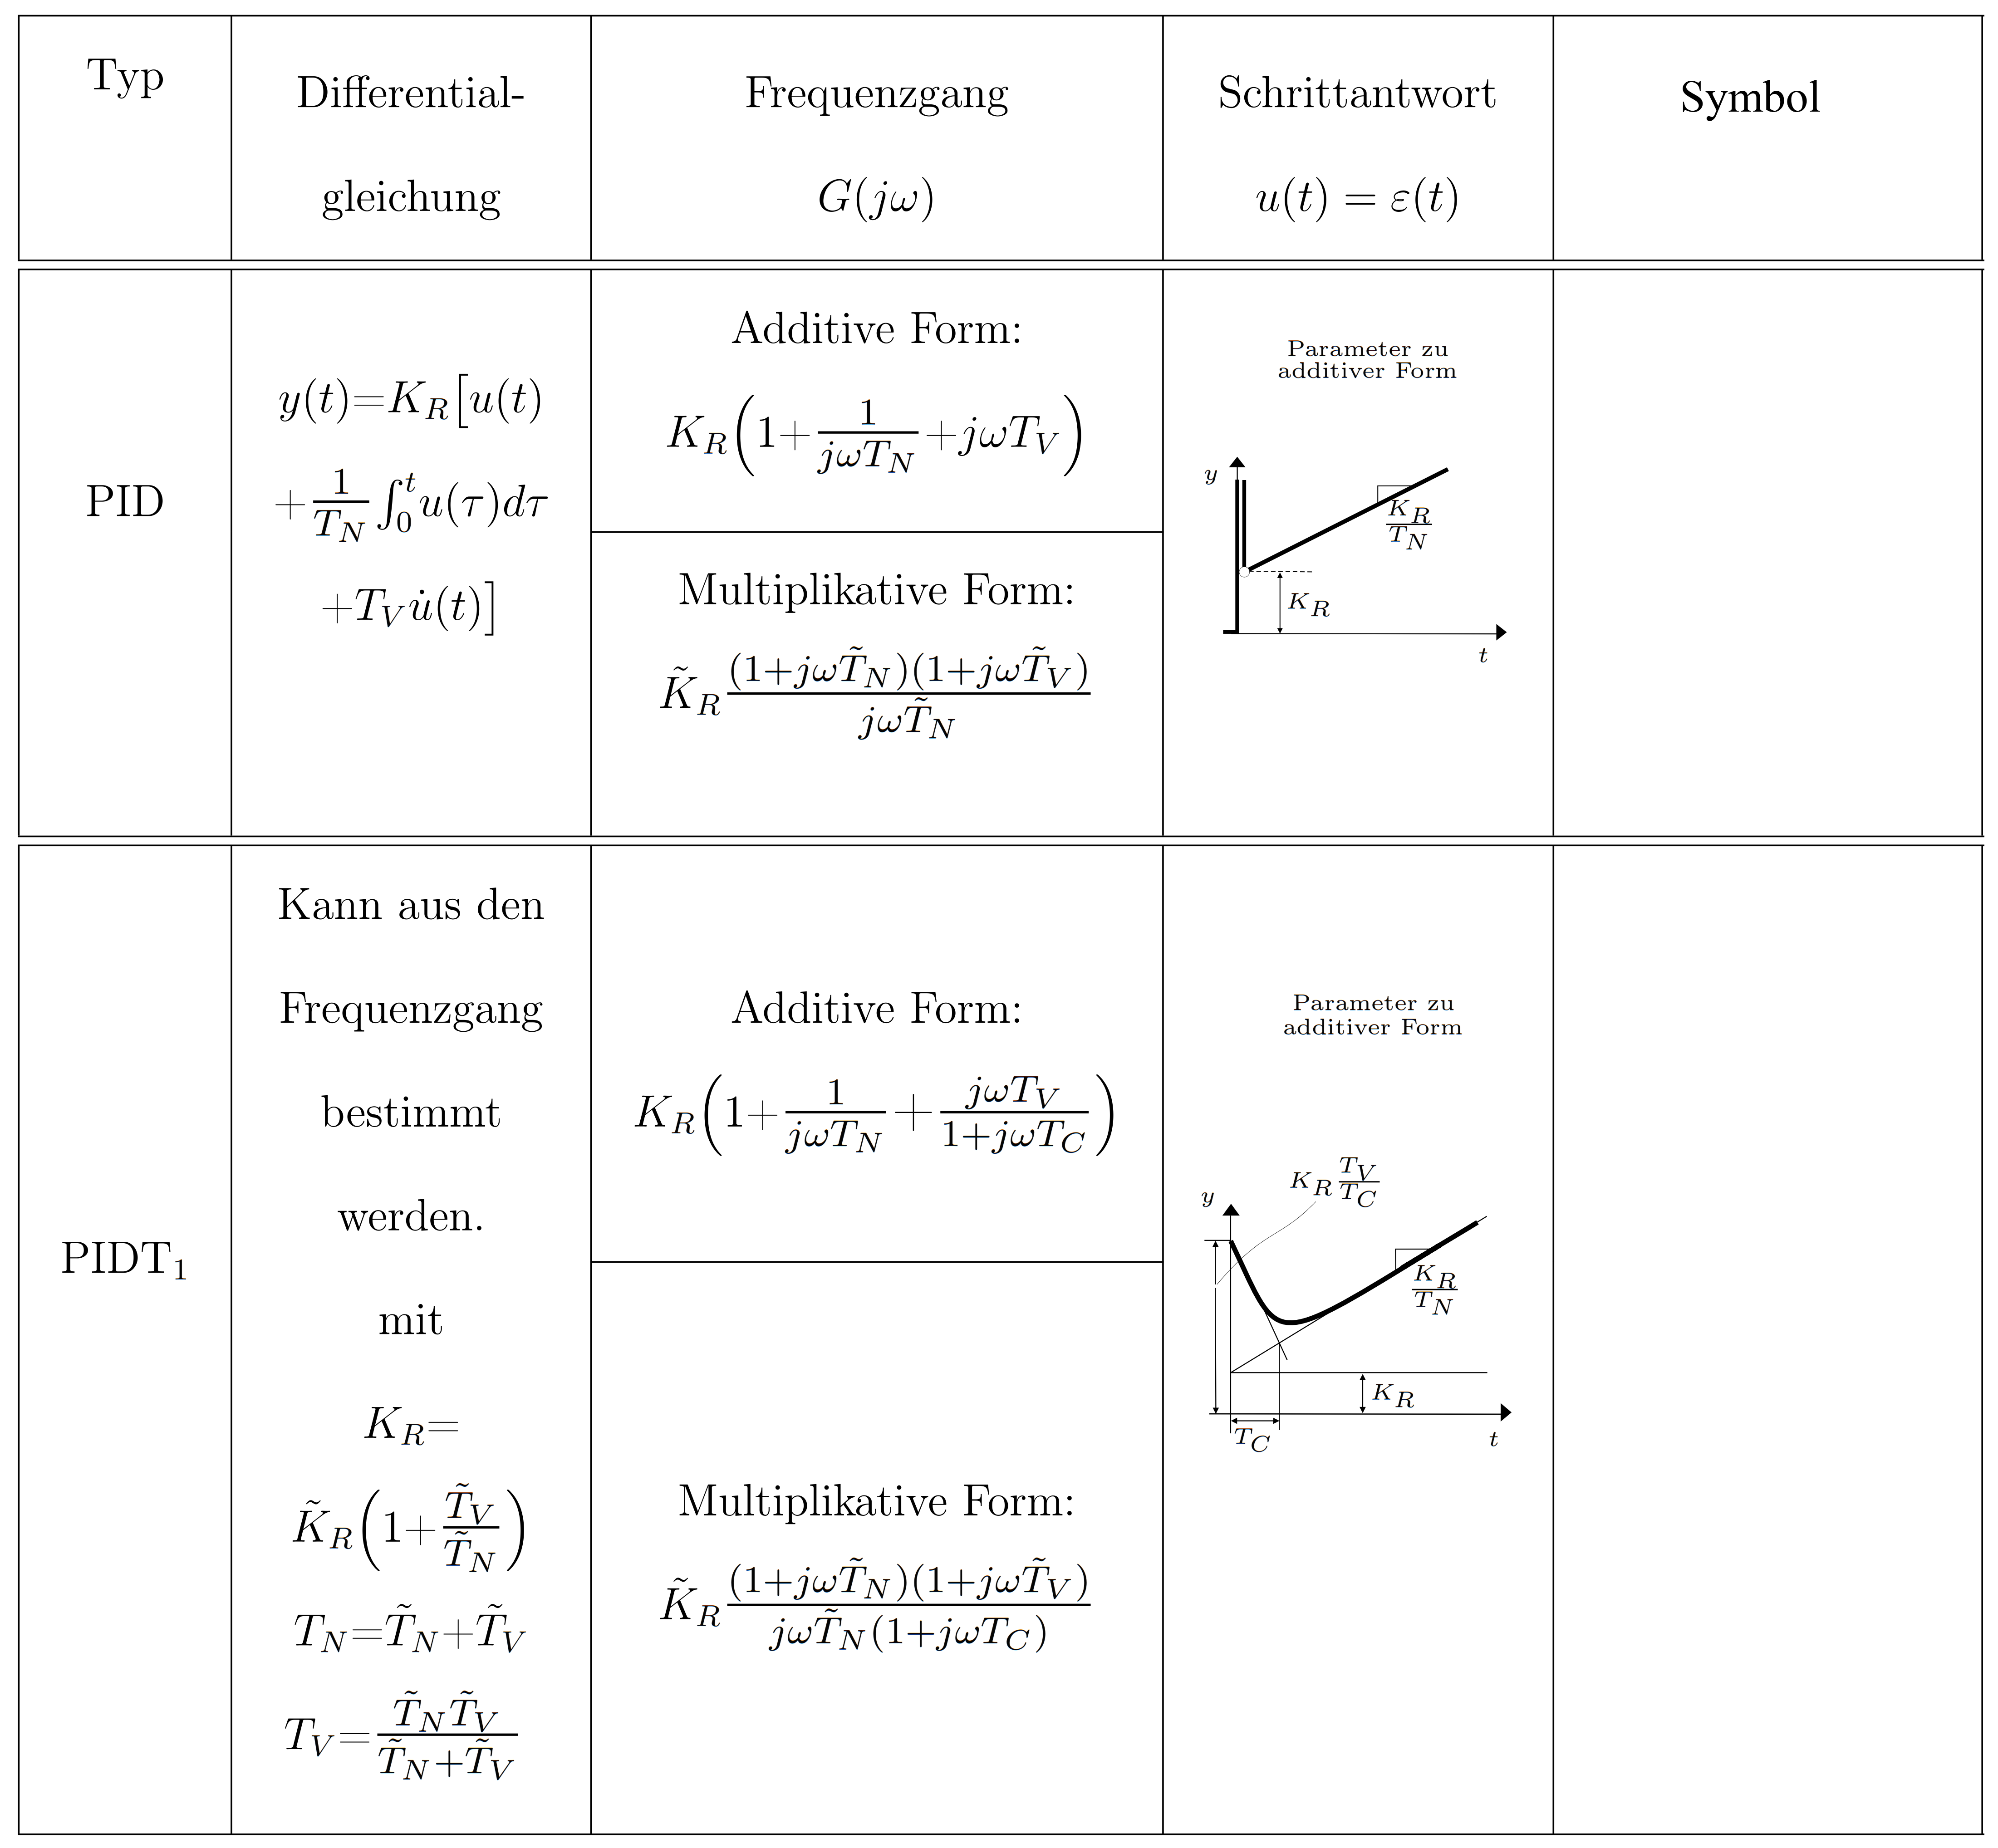
\includegraphics[width=13.5 cm]{./bilder/grundglieder/glieder5.png} \\






    \subsection {Elektronische Schaltungen}
    \begin{minipage}{7cm}
    \textbf{P-Glied (nicht inv. Op-Amp)}\\
    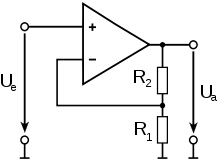
\includegraphics[height=2.5cm]{./bilder/OP-Amp.png} \\
    $K = 1 + \frac{R_2}{R_1}$
    \end{minipage}
    \begin{minipage}{6cm}
	\textbf{P-Glied (inv. Op-Amp)} \\ 
	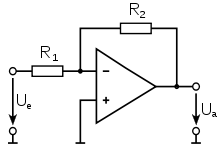
\includegraphics[height=2.5cm]{./bilder/OP-InvAmp.png} \\
	$K=-\frac{R_2}{R_1}$
    \end{minipage}
    \begin{minipage}{6cm}
	\textbf{I-Glied} \\ 
	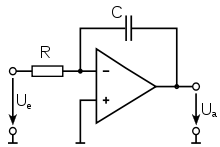
\includegraphics[height=2.5cm]{./bilder/OP-Integrator.png}\\
	$K = - \frac{1}{R \cdot C}$
    \end{minipage}  
    
		